\section{Serial Monitor}
\label{group__ro__monitor}\index{Serial Monitor@{Serial Monitor}}
A serial debug monitor.  
\subsection*{Defines}
\begin{CompactItemize}
\item 
\#define {\bf BUFLEN}~32
\end{CompactItemize}
\subsection*{Functions}
\begin{CompactItemize}
\item 
void {\bf monitor} ()
\end{CompactItemize}


\subsection{Detailed Description}
A serial debug monitor. 



\begin{Code}\begin{verbatim} #include <monitor.h> 
\end{verbatim}\end{Code}



The monitor program shows internal system-parameter and allows manipulations of variables

\begin{Desc}
\item[Note:]Based on Atmel Datasheet for Atmega128, Nov. 2006 \end{Desc}
\begin{Desc}
\item[Author:]Rainer Ostendorf \end{Desc}


\subsection{Define Documentation}
\index{ro_monitor@{ro\_\-monitor}!BUFLEN@{BUFLEN}}
\index{BUFLEN@{BUFLEN}!ro_monitor@{ro\_\-monitor}}
\subsubsection{\setlength{\rightskip}{0pt plus 5cm}\#define BUFLEN~32}\label{group__ro__monitor_gd974fe981249f5e84fbf1683b012c9f8}




Definition at line 49 of file monitor.h.

Referenced by monitor().

\subsection{Function Documentation}
\index{ro_monitor@{ro\_\-monitor}!monitor@{monitor}}
\index{monitor@{monitor}!ro_monitor@{ro\_\-monitor}}
\subsubsection{\setlength{\rightskip}{0pt plus 5cm}void monitor ()}\label{group__ro__monitor_g0e89037e727d646088e956504e02ef8b}




Definition at line 43 of file monitor.c.

References \_\-\_\-motor1\_\-duty, \_\-\_\-motor2\_\-duty, accl\_\-high\_\-samples, accl\_\-low\_\-samples, adc\_\-sel\_\-channel(), BUFLEN, gyro1\_\-samples, GYRO1\_\-SAMPLES\_\-BUFSIZE, gyro1\_\-temp, gyro2\_\-samples, gyro2\_\-temp, PWM\_\-RESOLUTION, read\_\-adc(), SYS\_\-CLK, uart\_\-puts(), and uart\_\-puts\_\-P.

Here is the call graph for this function:\begin{figure}[H]
\begin{center}
\leavevmode
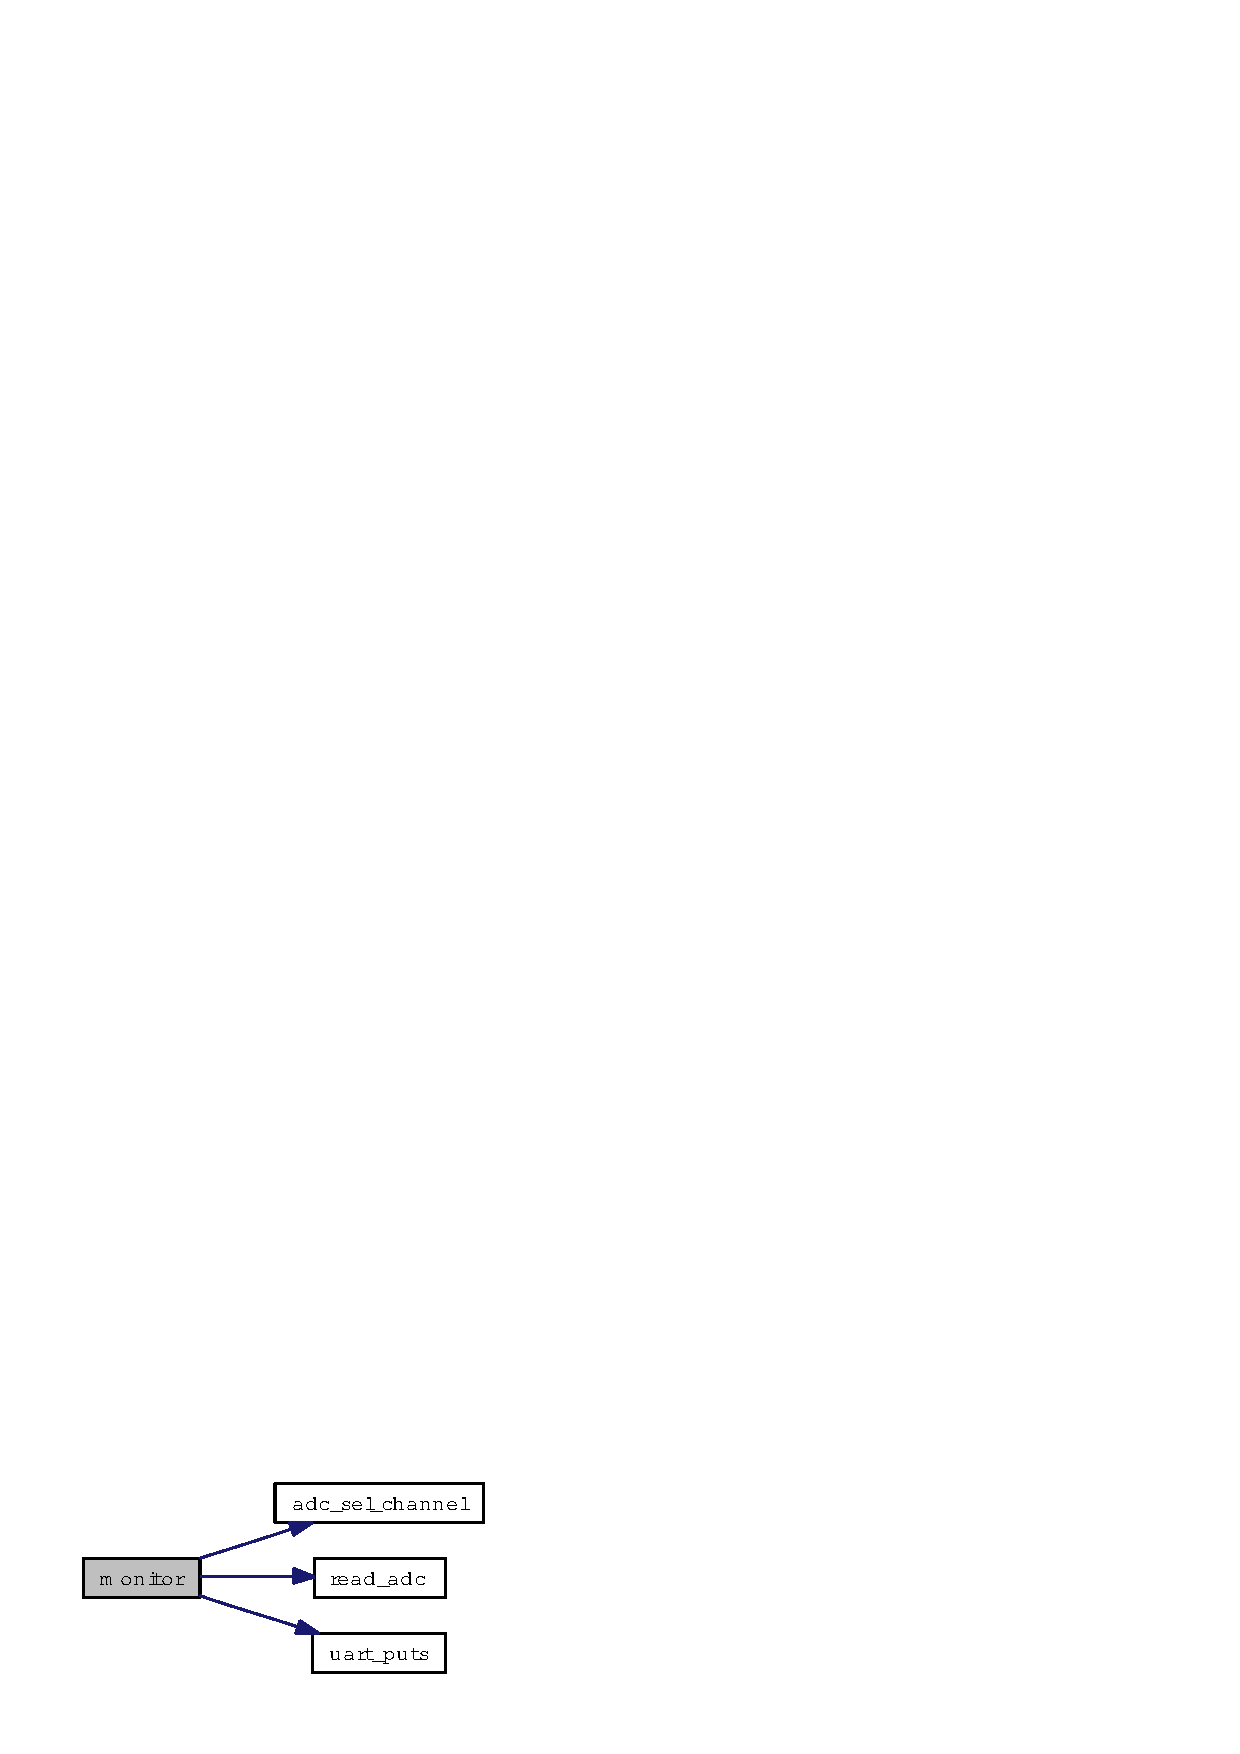
\includegraphics[width=118pt]{group__ro__monitor_g0e89037e727d646088e956504e02ef8b_cgraph}
\end{center}
\end{figure}
